\chapter{Logical Design}
\section*{Volumes Table}
We will consider a span of a month to evaluate the volumes of the entities.

\begin{table}[h!]
    \resizebox{\textwidth}{!}{
    \begin{tabular}{|l|c|p{14cm}|c|}
    \hline
    \textbf{Concept} & \textbf{Type} & \textbf{Computation} & \textbf{Final Volume} \\
    \hline
    Operational Center & E & 15 (assuming 10 team per \texttt{Operational Center}) & 15 \\
    \hline
    Linked To & R & 150 (same as \texttt{Team}) & 150 \\
    \hline
    Team & E & 150 (\textit{given}) & 150 \\
    \hline
    Handled By & R & 45000 (same as (assigned) \texttt{Order}) & 45000 \\
    \hline
    Order & E & $300 \; \text{op/m} \cdot 150 + 100 \; \text{not assigned}$ & 45100 \\
    \hline
    Belongs To & R & $150 \; \texttt{Team} \cdot 6.4 \; \text{current \texttt{Employee}}$ & 960 \\
    \hline
    Employee & E & $80\% \; \text{of} \; (150 \cdot 8) + 140 \; \text{past \texttt{Employee}}$ & 1100 \\
    \hline
    Manages & R & $45000 \cdot 3 \; \text{(assuming 3 \texttt{Employee} working on an \texttt{Order})}$ & 135000 \\
    \hline
    Places & R & $45100 \; \text{(same as \texttt{Order})}$ & 45100 \\
    \hline
    Business Account & E & $\dfrac{45100 \; \texttt{Order}}{1.5 \; \text{\texttt{Order}/month}}$ & 30000 \\
    \hline
    Have & R & $30000 \; \text{(same as \texttt{Business Account})}$ & 30000 \\
    \hline
    Customer & E & $\dfrac{30000 \; \texttt{Business Account}}{1.5 \; \text{\texttt{Business Account}/\texttt{Customer}}}$ & 20000 \\
    \hline
    Active Order & E & $20\% \; \text{of} \; 45000 + 100 \; \text{not assigned}$ & 9100 \\
    \hline
    Completed Order & E & $80\% \; \text{of} \; 45000$ & 36000 \\
    \hline
    Individual & E & $90\% \; \text{of \texttt{Customer}}$ & 18000 \\
    \hline
    Business & E & $10\% \; \text{of \texttt{Customer}}$ & 2000 \\
    \hline
    \end{tabular}
    }
\end{table}
    

\section*{Operations Analysis}
\begin{table}[H]
    \centering
    \begin{tabular}{|l|c|c|}
        \hline
        \textbf{Operation} & \textbf{Type} & \textbf{Frequency} \\
        \hline
        Operation 1 & I & 10/day \\
        \hline
        Operation 2 & I & 1000/day \\
        \hline
        Operation 3 & I & 500/day \\
        \hline
        Operation 4 & I & 200/day \\
        \hline
        Operation 5 & I & 20/day \\
        \hline
    \end{tabular}
    \caption{Operations frequency}
    \end{table}
    
    \textbf{Note}: we will double count the cost of writing operations.
    
    \subsection*{Operation 1: Register a new customer}
    
    \begin{table}[H]
    \centering
    \begin{tabular}{|l|c|c|c|}
    \hline
    \textbf{Concept} & \textbf{Type} & \textbf{No. Access} & \textbf{Access Type} \\
    \hline
    Customer         & E & 1 & W \\
    \hline
    Have             & R & 1 & W \\
    \hline
    Business Account & E & 1 & W \\
    \hline
    \end{tabular}
    \end{table}
    
    \textbf{Operation cost}: $6 \; \text{accesses} \cdot 10 = 60 \; \text{accesses/day}$
    
    \subsection*{Operation 2: Add a new order}
        
    \begin{table}[h!]
        \centering
        \begin{tabular}{|l|c|c|c|}
        \hline
        \textbf{Concept} & \textbf{Type} & \textbf{No. Access} & \textbf{Access Type} \\
        \hline
        Order   & E & 1 & W \\
        \hline
        Places  & R & 1 & W \\
        \hline
        \end{tabular}
    \end{table}
        
    \textbf{Operation cost}: $4 \; \text{accesses} \cdot 1000 = 4000 \; \text{accesses/day}$
    \subsection*{Operation 3: Assign an order to a management team}
    
    Access \textit{without} redundancy \texttt{Team.NoOrders}:
    
    \begin{table}[h!]
    \centering
    \begin{tabular}{|l|c|c|c|}
    \hline
    \textbf{Concept} & \textbf{Type} & \textbf{No. Access} & \textbf{Access Type} \\
    \hline
    Handled By & R & 1 & W \\
    \hline
    Manages    & R & 3 & W \\
    \hline
    \end{tabular}
    \end{table}
    
    Access \textit{with} redundancy \texttt{Team.NoOrders}:
    
    \begin{table}[h!]
    \centering
    \begin{tabular}{|l|c|c|c|}
    \hline
    \textbf{Concept} & \textbf{Type} & \textbf{No. Access} & \textbf{Access Type} \\
    \hline
    Handled By & R & 1 & W \\
    \hline
    Team       & E & 1 & R \\
    \hline
    Team       & E & 1 & W \\
    \hline
    Manages    & R & 3 & W \\
    \hline
    \end{tabular}
    \end{table}
    
    \textbf{Operation cost} (\textit{without redundancy}): $8 \; \text{accesses} \cdot 500 = 4000 \; \text{accesses/day}$ 

    \textbf{Operation cost} (\textit{with redundancy}): $11 \; \text{accesses} \cdot 500 = 5500 \; \text{accesses/day}$
    
    \subsection*{Operation 4A: View the total number of operations handled by a specific team}
    
    Access \textit{with} redundancy \texttt{Team.NoOrders}:
    
    \begin{table}[h!]
    \centering
    \begin{tabular}{|l|c|c|c|}
    \hline
    \textbf{Concept} & \textbf{Type} & \textbf{No. Access} & \textbf{Access Type} \\
    \hline
    Team    & E & 1 & R \\
    \hline
    \end{tabular}
    \end{table}
    
    Access \textit{without} redundancy \texttt{Team.NoOrders}:
    
    \begin{table}[h!]
    \centering
    \begin{tabular}{|l|c|c|c|}
    \hline
    \textbf{Concept}    & \textbf{Type} & \textbf{No. Access} & \textbf{Access Type} \\
    \hline
    Handled By & R & 300 & R \\
    \hline
    \end{tabular}
    \end{table}
    
    \textbf{Operation cost} (\textit{without redundancy}): $300 \; \text{accesses} \cdot 200 = 60000 \; \text{accesses/day}$

    \textbf{Operation cost} (\textit{with redundancy}): $1 \; \text{access} \cdot 200 = 200 \; \text{accesses/day}$  

    \subsection*{Operation 4B: Show the total cost of the orders handled by a specific team}
    Access \textit{with} redundancy \texttt{Team.NoOrders}:
    
    \begin{table}[H]
        \centering
        \begin{tabular}{|l|c|c|c|}
        \hline
        \textbf{Concept} & \textbf{Type} & \textbf{No. Access} & \textbf{Access Type} \\
        \hline
        Team    & E & 1 & R \\
        \hline
        \end{tabular}
        \end{table}
    
        Access \textit{without} redundancy \texttt{Team.NoOrders}:
    
    \begin{table}[h!]
        \centering
        \begin{tabular}{|l|c|c|c|}
            \hline
            \textbf{Concept} & \textbf{Type} & \textbf{No. Access} & \textbf{Access Type} \\
            \hline
            Team    & E & 1 & R \\
            \hline
            Handled & R & 300 & R \\
            \hline
            Order  & E & 300 & R \\
            \hline
        \end{tabular}
    \end{table}
    
    \textbf{Operation cost} (\textit{without redundancy}): $601 \; \text{accesses} \cdot 200 = 60000 \; \text{accesses/day}$

    \textbf{Operation cost} (\textit{with redundancy}): $1 \; \text{access} \cdot 200 = 200 \; \text{accesses/day}$  


    \subsection*{Operation 5: Print a list of teams sorted by their performance score}
    
    Access \textit{with} redundancy \texttt{Team.PerformanceScore}:
    
    \begin{table}[h!]
    \centering
    \begin{tabular}{|l|c|c|c|}
    \hline
    \textbf{Concept} & \textbf{Type} & \textbf{No. Access} & \textbf{Access Type} \\
    \hline
    Team    & E & 150 & R \\
    \hline
    \end{tabular}
    \end{table}
    
    Access \textit{without} redundancy \texttt{Team.PerformanceScore}:
    
    \begin{table}[h!]
    \centering
    \begin{tabular}{|l|c|c|c|}
    \hline
    \textbf{Concept} & \textbf{Type} & \textbf{No. Access} & \textbf{Access Type} \\
    \hline
    Team       & E & 150    & R \\
    \hline
    Handled By & R & 45000  & R \\
    \hline
    Order      & E & 45000  & R \\
    \hline
    \end{tabular}
    \end{table}
    
    \textbf{Operation cost} (\textit{without redundancy}): $90150 \; \text{accesses} \cdot 20 = 1803000 \; \text{accesses/day}$

    \textbf{Operation cost} (\textit{with redundancy}): $150 \; \text{accesses} \cdot 20 = 3000 \; \text{accesses/day}$  

    

\section*{Redundancy Analysis}
\begin{itemize}[label=-]
\item \texttt{OperationalCenter.NoEmployees}: Since no operations utilize this attribute, we decide to \textbf{eliminate} this redundancy.
\item \texttt{Team.NoOrders}: The analysis shows 5,900 accesses with redundancy versus 124,000 accesses without redundancy when combining Operations (3), (4A), and (4B). Based on this significant difference, we decide to \textbf{maintain} this redundancy.
\item \texttt{Team.PerformanceScore}: Operation (5) requires 3,000 accesses with redundancy compared to 1,803,000 accesses without it. Given this substantial performance impact, we decide to \textbf{maintain} this redundancy.
\end{itemize}


\section*{Partitioning and Merging}
\begin{itemize}[label=-]
    \item Merging \texttt{Active Order} and \texttt{Completed Order} into \texttt{Order}: since no operations require distinguishing between these two entities, we can \textbf{merge} them into a single entity.
    \item Merging \texttt{Individual} and \texttt{Business} into \texttt{Customer}: since no operations require distinguishing between these two types of customers, we can \textbf{merge} them into a single entity.
\end{itemize}

\subsection*{Restructured Schema}
\begin{figure}[H]
    \centering
    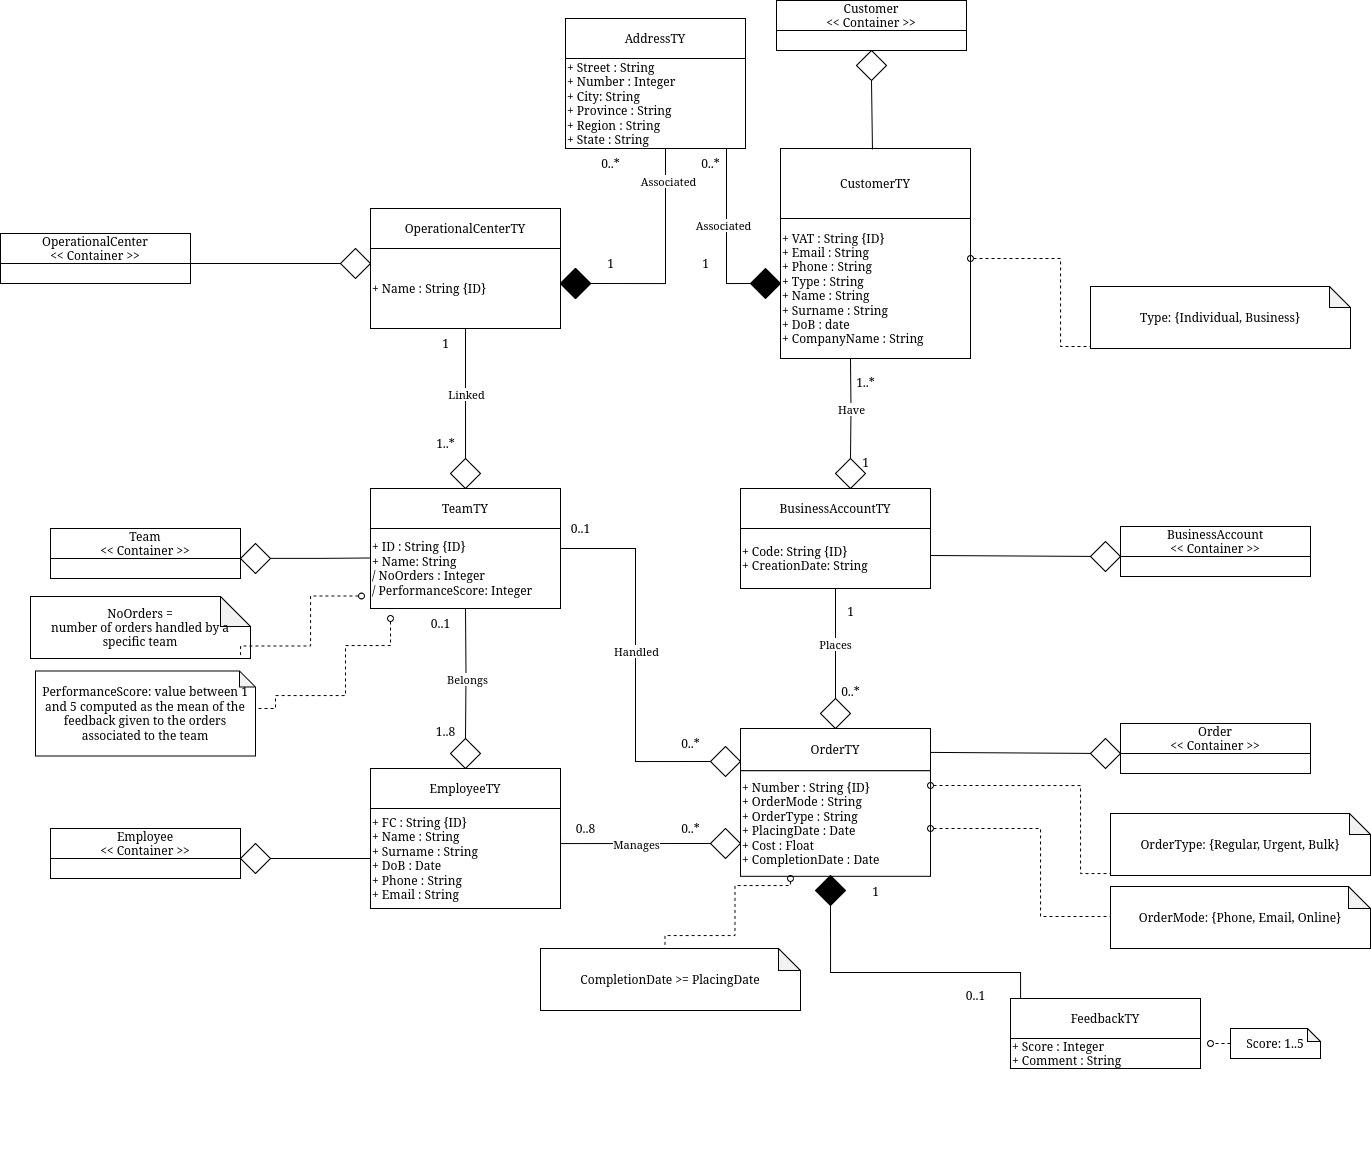
\includegraphics[width=0.8\textwidth]{img/UML.jpg}
\end{figure}

\subsection*{Other Details}
\begin{itemize}[label=-]
    \item When an Operational Center is deleted, the associated teams are also deleted, causing dereferencing of the orders linked to these teams.
    \item When a Customer is deleted, the associated business accounts are also deleted, causing dereferencing of the orders linked to these accounts.
    \item As a result of the previous observations, an order can be deleted only if there are not information for the business account (order history) or for the feedback computation.
    \item The existence of a completion date in a order mark the order as completed, otherwise is active.
    \item After a team is updated on an order, the list of employees is cleared.
    \item We use AddressTY to define the composite attribute Address in OperationalCenterTY and CustomerTY.
\end{itemize}